\section{Part 2: isolate correction and feedback}
Part 1 changes restraint and query horizon together. Its failure investigation
found some corrected commands followed by cached proposals, motivating a bounded
mechanism test rather than an established diagnosis. Four conditions use the same
frozen VLA: A preserves its commands and queries every eight actions; B applies the
finalist's .04/.02 rad caps at interval eight; C uses those caps at interval four;
D uses those caps with correction-triggered refresh between four and eight. The
finger heuristic, componentwise mapping and smoothing one are common to B/C/D.
There is no new evolutionary search or three-setting dial sweep in Part 2.

After actual environment input $u_t$, D accumulates
\begin{equation}
 D_k=\sum_{t\text{ since query}}
 \frac{\|p_t^{\rm arm}-u_t^{\rm arm}\|_2}{\sqrt7\,(.04\text{ rad})}.
\end{equation}
Per-coordinate differences no larger than $10^{-6}$ rad are zeroed first. The
accumulator resets on a query, preserving previous actual input and finger history.
Goal termination takes precedence; otherwise refresh occurs once $k\ge4$ and
$D_k\ge.5$, or at $k=8$. Both the correction and trigger use already executed
inputs after downstream action-space clipping. Command departure measures neither
actual displacement nor physical risk. No privileged held label, object pose or
monitor verdict enters this controller.

The frozen allocation has sixteen full episodes: tasks 0039/0010 each receive two
fresh base seeds (4000/4001 and 4010/4011), with four conditions in each matched block.
The prospective order is ABCD, BCDA, CDAB, DABC. Native horizon, goals, monitor and
policy inference remain unchanged. Engineering checks A/C/D at 32 actions each;
one pre-application import failure and two coordinator/tooling failures are retained.
There are no full-episode retries or outcome-dependent additions.

\subsection{Part 2 measured outcomes}
All sixteen full episodes pass independent action/monitor replay, source/checkpoint
and native sampling-seed checks. Safe completion is 3/4 for A, B and D and 2/4 for C;
each condition has one violating episode (Figure~\ref{fig:part2-outcomes}). Requested
completion is 3/4 in every condition. A/B/D each have one unsafe unfinished episode;
C has one unsafe completion and one safe unfinished episode. All conditions safely
complete both task 0010 episodes. On task 0039, A/B/D each safely complete one of two,
whereas C safely completes neither. These small descriptive counts support no claim
that one schedule is superior or that frequent feedback itself causes harm.

\begin{figure*}[t]
\centering
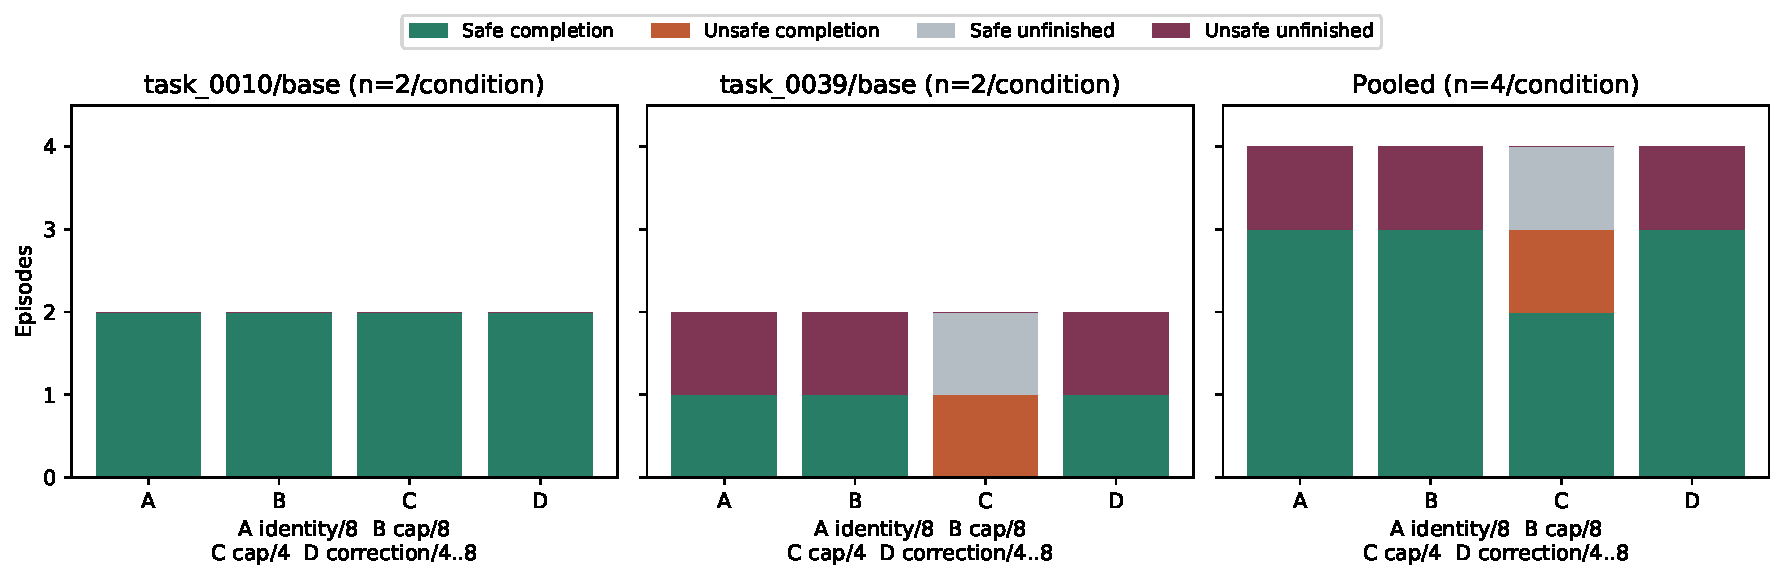
\includegraphics[width=\textwidth]{part2-outcomes.pdf}
\caption{Part 2's complete sixteen-episode sample, with unsafe completion and both
unfinished categories preserved. Each scene has two episodes per condition; pooled
denominators are four. A is identity/8, B is cap/8, C is cap/4 and D is correction/4--8.}
\Description{Pooled safe completions are three, three, two and three of four.
Every condition has one violating episode; only C completes unsafely.}
\label{fig:part2-outcomes}
\end{figure*}

The adaptive rule never changes the query schedule: every one of D's 337 actual
inter-query intervals is eight actions (Figure~\ref{fig:part2-feedback}). Its correction
threshold is crossed once, at action eight, when a query is already due. There is no
crossing at actions four through seven. Its largest accumulated correction is .60146.
Thus this run supplies no adaptive-feedback gain while leaving an actively triggering
rule untested. The threshold is retained rather than adjusted against these outcomes.
C uses 750 queries versus B's 336 without improving measured safe completion.

\begin{figure*}[t]
\centering
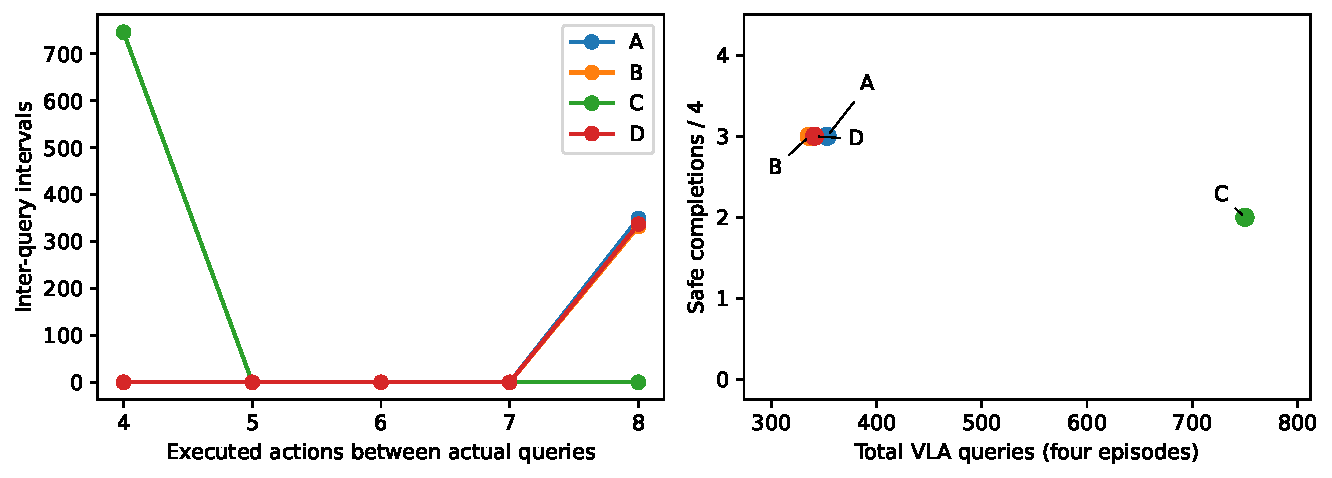
\includegraphics[width=.85\textwidth]{part2-feedback.pdf}
\caption{Observed inter-query intervals and query cost in Part 2. A/B/D always wait
eight actions; C always waits four. Safe completions have denominator four.}
\Description{The adaptive controller D shares the fixed-eight schedule, while fixed
four more than doubles queries without increasing safe completions.}
\label{fig:part2-feedback}
\end{figure*}

\begin{table}[t]
\caption{Part 2 costs. Time is measured inside each evaluator, including capture;
outer process time over all sixteen episodes is 1,897.69 s.}
\label{tab:part2-costs}
\begin{tabular}{lrrrr}
\toprule
Condition & Actions & Queries & Time (s) & Corrections \\
\midrule
A & 2,810 & 353 & 455.13 & 0 \\
B & 2,674 & 336 & 438.27 & 76 \\
C & 2,992 & 750 & 499.49 & 55 \\
D & 2,714 & 341 & 451.85 & 54 \\
\bottomrule
\end{tabular}
\end{table}

Table~\ref{tab:part2-costs} counts substantial arm changes above $10^{-6}$ rad.
Exact changed-command counters are 0/122/95/92; the additional numerical changes
are roundoff rather than further substantial cap activations. All four episodes per
condition show contact; grasp flags occur in 4/4 for A and 3/4 for B/C/D. Such flags
do not establish successful continuation after contact.

All twelve initial robot-state comparisons against A are exactly equal, but none of
the corresponding 24 camera pairs or twelve first chunks is exactly equal. Matched
scene and sampling-seed settings therefore do not identify single-episode causal
counterfactuals. The prescribed fixed-reference selection chooses B, with mean
$U=.25$ versus C's zero; no additional setting is tuned.

The full sample records 11,190 controls, 1,780 queries and 68,516 post-subscription
physics ticks. Engineering adds 96 controls, sixteen queries and 834 known ticks;
the pre-application failure retains unknown native counters. Synthetic CPU checks
precede engineering, but recorded physical-input replay first audits engineering
jobs rather than preceding them as requested by the plan. This chronology deviation
is explicit; all engineering replay passes before the full comparison freeze.
Twenty-four targeted CPU checks pass across Parts 2 and 3. Every native camera clip,
all eight matched Part 2 videos and complete event-picture strips are preserved.


\section{Part 3: model feasibility before evolutionary use}
The proposed contribution concerns which motion mutants merit physical evaluation,
using observed errors conditional on execution correction. Dynamics-assisted
skill search already exists~\cite{daqd}; frozen visual-feature prediction and short
rollouts also have precedent~\cite{dinowm,mbpo}. These ingredients and an optimizer
substitution do not establish novelty. We test a compact feasibility stage before
spending the physical optimizer-comparison allocation.

\paragraph{Data and information.}
The Part 1 training traces lack later exact images and numerical margins; exposed
Part 1 comparison episodes are excluded. Before fitting, the declared eight-episode
recording option is sealed: B/C on tasks 0046/0006, two fresh seeds per task. All
sixteen Part 2 episodes on 0039/0010 are fitting data; four 0046 episodes calibrate;
four 0006 episodes audit. Whole tasks, seeds and trajectories remain separated.
The 0048/0050 final comparison and main-study test partition are outside development.
Acquisition is charged once, including reused common data.

Passive capture, identical across all Part 2/3 recording conditions, saves the
already extracted overview/wrist RGB at every step without rendering or advancing
physics. Evaluation-only numerical targets reproduce the native float32 local
$+Z$ tilt calculation and per-object thresholds, plus negative target-to-goal
distance. Targets never enter the live controller or dynamics input. Numerical
uprightness is audited against native Boolean bindings. The final image remains
saved but is omitted from model pairs without its missing subsequent two-finger
proposal frame. A spatial distance readout is distinct from the native held-object
goal; tilt is distinct from spill/drop safety.

\paragraph{Frozen predictive system.}
A pinned DINOv2 small encoder~\cite{dinov2} produces $2\times2$ spatially pooled
patch features from each camera, 3,072 coordinates in total. Fitting-only
standardization and randomized PCA retain 32 visual coordinates. Seven measured
arm joints and both finger positions remain separate. Five episode-bootstrap
128/128-unit residual MLPs predict the next standardized visual/robot state,
conditioned on the current and previous state and previous/current actual
8-coordinate environment inputs. Each trains for 30 epochs with fixed settings.
History shifts causally during rollouts of at most four actions. PCA is compression;
the action-conditioned residual networks supply the dynamics.

Ridge heads estimate minimum upright margin and short-term progress. The audit
compares persistence, fitted ridge, action-shuffled ridge and the same ensemble
with mispaired action sequences, changing-state windows, and actual versus
predicted future-state readouts. Raw pooled features, PCA and a same-size random
projection diagnose representation/readout limitations. Correctly paired and
shuffled sequences share the same trained ensemble in the action-dependence gate.
Pre-fitting source refinements preserve their original receipts; numerical criteria,
data groups, physical slots and model hyperparameters are unchanged.

\paragraph{Reliability and prospective search.}
M trusts ensemble disagreement; C uses an empirical conditional .8-error-quantile
lookup by factual correction, with sparse bins falling back to the unconditional
quantile and unsupported contexts abstaining. Both use nominal .5 calibration
acceptance; actual acceptance and consequential errors must also be reported.
These are empirical allocation heuristics, not calibrated safety probabilities.
Planned counterfactual correction never becomes a factual residual without execution.

If the sealed forecast criteria permit, the 64-episode physical pilot evaluates a
shared four-controller initial population on two cases (eight episodes once),
three four-slot descendant populations on two fresh cases (24), two shortlisted
controllers per method on two confirmation cases (12), and identity, one fixed
Part 2 reference and three frozen finalists on four fresh blocks (20). Each
method retains an actually re-evaluated elite, one unguided timing mutant and
two cap mutants from a common pool of at most sixteen proposals. The known
four-command prefix cannot rank later query timing, so timing genes stay in
physical exploration. Abstention removes a model recommendation rather than a
candidate's exploration eligibility. All deployed controllers share the same
information and family; actual mean $U$ determines selection and confirmation.
No learned online action veto is installed. Three additional 32-action engineering
attempts are available before eligible search, with no full-episode replacement.
The deployed family has 160 genotypes: free caps
$\{\varnothing,.12,.08,.04\}$ rad, grasp caps
$\{\varnothing,.08,.04,.02\}$ rad, thresholds $\{0,.5,1,2,\varnothing\}$,
and minimum intervals $\{4,6\}$, with maximum eight and smoothing one fixed.
